\section{Preventing Goodharting Behaviour}\label{sec:preventing_goodhart}

\begin{figure}[]
    % \vspace{-3mm}
    \centering
    \begin{subfigure}[b]{0.40\textwidth}
        \centering
        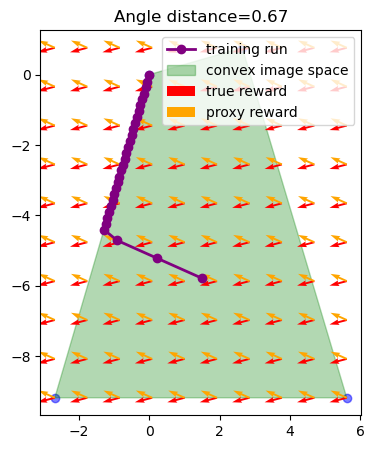
\includegraphics[width=0.65\linewidth]{example/example_sa_trajectory.png}
        \caption{A $\occmeas{\phantom{}}$-embedded training run for steepest ascent. The training curve is split into two linear segments: the first is parallel to the proxy reward, while the second is parallel to the proxy reward projected onto some boundary plane $\plane$. Goodharting only occurs along $\plane$. (Compare to the MCE approximation of Steepest Ascent in~\Cref{subfig:2-2-mce-image})}
        \label{fig:fig:2-2-SA-explanation}
    \end{subfigure}
    \hfill
        \begin{subfigure}[b]{0.56\textwidth}
    \begin{framed}
        \begin{algorithmic}
            \Procedure{EarlyStopping}{$\S, \A, \T, \AngBound, \R$}
              \State $\vec{r} \gets \QProj_\T \R$
              \State $\policy \gets Unif[\RR^{\SxA}]$
              \State $\vec{\occmeaselem}_0 \gets \occmeas{\policy}$
              \State $\TangentVec_0 \gets \amax_{\TangentVec \in \ConeTangent(\vec{\occmeaselem}_0)} \TangentVec \cdot \VecR$
              \While{$ (\vec{t}_i \neq \vec{0}) \textbf{ and } \VecR \cdot \TangentVec_{i} \leq \sin(\AngBound)||\VecR|| $}
                \State $\lambda \gets \max \{\lambda:\vec{\occmeaselem}_i+\lambda \TangentVec_i \in \Polytope\}$
                \State $\vec{\occmeaselem}_{i+1} \gets \vec{\occmeaselem}_i + \lambda \TangentVec_i$
                \State $\TangentVec_{i+1} \gets \amax_{\TangentVec \in \ConeTangent(\vec{\occmeaselem}_{i+1})} \TangentVec \cdot \VecR$
                \State $i \gets i + 1$
              \EndWhile
              \State \Return $(\occmeas{\vec{\occmeaselem}_i})^{-1}$
            \EndProcedure
        \end{algorithmic}
        \end{framed}
        \caption{Early stopping pseudocode for Steepest Ascent. Given the correct $\theta$, the algorithm would stop at the point where the training run hits the boundary of the convex hull. The cone of tangents, $T(\occmeaselem)$ is defined in \cite{denel_steepest_1981}.}
        \label{alg:early-stopping-code}
    \end{subfigure}
    \caption{Early stopping algorithm and its behaviour.}
    \label{fig:sa-example-run}
    \vspace{-4mm}
\end{figure}



We have seen that when a proxy reward $\ProxR$ is optimised, it is common for the true reward $\TrueR$ to first increase, and then decrease. 
If we can stop the optimisation process before $\TrueR$ starts to decrease, then we can avoid Goodharting.
Our next result shows that we can \emph{provably} prevent Goodharting, given that we have a bound $\theta$ on the distance between $\ProxR$ and $\TrueR$:

\begin{theorem}\label{thm:optimal_stopping}
Let $\ProxR$ be any reward function, let $\theta \in [0,\pi]$ be any angle, and let $\pi_A, \pi_B$ be any two policies. Then there exists a reward function $\TrueR$ with $\Angle{\TrueR}{\ProxR} \leq \AngBound$ and $\J_{\TrueR}(\policy_A) > \J_{\TrueR}(\policy_B)$ iff
$$
\frac{\J_{\ProxR}(\policy_B)-\J_{\ProxR}(\policy_A)}{||\occmeas{\policy_B}-\occmeas{\policy_A}||} < \sin(\AngBound)||\QProj_\T \ProxR||
$$
\end{theorem}
\begin{corollary}[Optimal Stopping]\label{cor:optimal_stopping}
Let $\ProxR$ be a proxy reward, and let $\{\policy_i\}$ be a sequence of policies produced by an optimisation algorithm. Suppose the optimisation algorithm is concave with respect to the policy, in the sense that $\frac{\J_{\ProxR}(\policy_{i+1})-\J_{\ProxR}(\policy_{i})}{||\occmeas{\policy_{i+1}}-\occmeas{\policy_{i}}||}$ is decreasing.
Then, stopping at minimal $i$ with 
$$
\frac{\J_{\ProxR}(\policy_{i+1})-\J_{\ProxR}(\policy_{i})}{||\occmeas{\policy_{i+1}}-\occmeas{\policy_{i}}||} < \sin(\AngBound)||\QProj_\T \ProxR||
$$
gives the policy $\pi_i \in \{\policy_i\}$ that maximizes 
$\min_{\TrueR \in \FeasibleR^\RMag}\J_{\TrueR}(\pi_i)$,
where $\FeasibleR^\RMag$ is the set of rewards given by $\{\TrueR:\Angle{\TrueR}{\ProxR}\leq \AngBound, ||\QProj_\T\TrueR|| = \RMag\}$.
\end{corollary}

Let us unpack the statement of this result. 
If we have a proxy reward $\ProxR$, and we believe that the angle between $\ProxR$ and the true reward $\TrueR$ is at most $\AngBound$, then $\FeasibleR^\RMag$ is the set of all possible true reward functions with a given magnitude $m$. 
Note that no generality is lost by assuming that $\TrueR$ has magnitude $m$, since we can rescale any reward function without affecting its policy order.
Now, if we optimise $\ProxR$, and want to provably avoid Goodharting, then we must stop the optimisation process at a point where there is no Goodharting for any reward function in $\FeasibleR^\RMag$.
Theorem~\ref{thm:optimal_stopping} provides us with such a stopping point. Moreover, if the policy optimisation process is concave, then Corollary~\ref{cor:optimal_stopping} tells us that this stopping point, in a certain sense, is worst-case optimal.
By Proposition~\ref{prop:concave_proof}, we should expect most optimisation algorithms to be approximately concave. 


\Cref{thm:optimal_stopping} derives an optimal stopping point among a single optimisation curve. Our next result finds the optimum among \textit{all} policies through maximising a regularised objective function.

\begin{proposition}\label{thm:regularised_reward}
    Given a proxy reward $\ProxR$, let $\FeasibleR^\RMag$ be the set of possible true rewards
    $\R$ such that 
    $\Angle{\R}{\ProxR} \leq \theta$ and $\R$ is normalized so that $||\QProj_\T \R|| = ||\QProj_\T \ProxR||$. Then, a policy $\policy$ maximises $\min_{\R \in \FeasibleR^\RMag}\J_{\R}(\policy)$ if and only if it maximises $\J_{\ProxR}(\policy)- \kappa ||\occmeas{\policy}|| \sin\left(\Angle{\occmeas{\policy}}{\ProxR}\right)$,
    where 
    $\kappa = \tan(\AngBound)||\QProj_\T\ProxR||$. Moreover, each local maximum of this objective is a global maximum when restricted to $\Omega$, giving that this function can be practically optimised for.
\end{proposition}

The above objective can be rewritten as 
$||\vec{\occmeaselem}_{\parallel}||-\kappa||\vec{\occmeaselem}_{\perp}||$
where $\vec{\occmeaselem}_{\parallel}, \vec{\occmeaselem}_{\perp}$ are the components of $\occmeas{\policy}$ parallel and perpendicular to $\QProj_\T\ProxR$. 

Stopping early clearly loses proxy reward, but it is important to note that it may also lose true reward. Since the algorithm is pessimistic, the optimisation stops before \textit{any} reward in $\FeasibleR^\RMag$ decreases. If we continued ascent past this stopping point, exactly one reward function in $\FeasibleR^\RMag$ would decrease (almost surely), but most other reward function would increase. If the true reward function is in this latter set, then early stopping loses some true reward. Our next result gives an upper bound on this quantity:

\begin{proposition}%[]
Let $\TrueR$ be a true reward and $\ProxR$ a proxy reward such that $\|\TrueR\| = \|\ProxR\| = 1$ and $\Angle{\TrueR}{\ProxR} = \AngBound$, and assume that the steepest ascent algorithm applied to $\ProxR$ produces a sequence of policies $\policy_0, \policy_1, \dots \policy_n$. If $\OptimalPolicy$ is optimal for $\TrueR$, we have that
$$
\J_{\TrueR}(\OptimalPolicy) - \J_{\TrueR}(\policy_{n}) \leq 
\mathrm{diameter}(\Omega) - \| \occmeas{\policy_{n}} - \occmeas{\policy_{0}}\|\cos(\AngBound).
$$
\end{proposition}

It would be interesting to develop policy optimisation algorithms that start with an initial estimate $\ProxR$ of the true reward $\TrueR$ and then refine $\ProxR$ over time as the ambiguity in $\ProxR$ becomes relevant.
Theorems~\ref{thm:optimal_stopping} and \ref{thm:regularised_reward} could then be used to check when more information about the true reward is needed. While we mostly leave this for future work, we carry out some initial exploration in~\Cref{appendix:iterative_improvement}.





\subsection{Experimental Evaluation of Early Stopping}\label{sec:evaluation}


We evaluate the early stopping algorithm experimentally. One problem is that Algorithm~\ref{alg:early-stopping-code} involves the projection onto $\Polytope$, which is infeasible to compute exactly due to the number of deterministic policies being exponential in $|S|$. Instead, we observe that using MCE and BR approximates the steepest ascent trajectory.

Using the exact setup described in~\Cref{subsect:estimating-prevalence}, we verify that \emph{the early stopping procedure prevents Goodharting in all cases}, that is, employing the criterion from~\Cref{cor:optimal_stopping} always results in NDH = 0. Because early stopping is pessimistic, some reward will usually be lost. We are interested in whether the choice of (1) operationalisation of optimisation pressure, (2) the type of environment or (3) the angle distance $\theta$ impacts the performance of early stopping.
%
A priori, we expected the answer to the first question to be negative and the answer to the third to be positive. ~\Cref{fig:evaluation-envs} shows that, as expected, the choice between MCE and Boltzmann Rationality has little effect on the performance. Unfortunately, and somewhat surprisingly, the early stopping procedure can, in general, lose out on a lot of reward; in our experiments, this is on average between $10\%$ and $44\%$, depending on the size and the type of environment. The relationship between the distance and the lost reward seems to indicate that for small values of $\theta$, the loss of reward is less significant (c.f. \Cref{fig:evaluation-theta}).


\begin{figure}[t]
    \centering
    \begin{subfigure}[b]{0.39\textwidth}
        \centering
        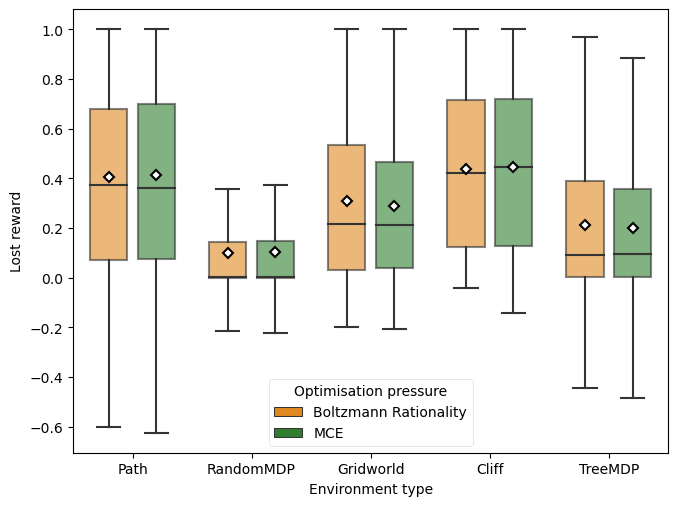
\includegraphics[width=1\linewidth]{lost_reward_plots/boxplot_52.png}
        \caption{}
        \label{fig:evaluation-envs}
    \end{subfigure}
    \hfill
    \begin{subfigure}[b]{0.55\textwidth}
        \centering
        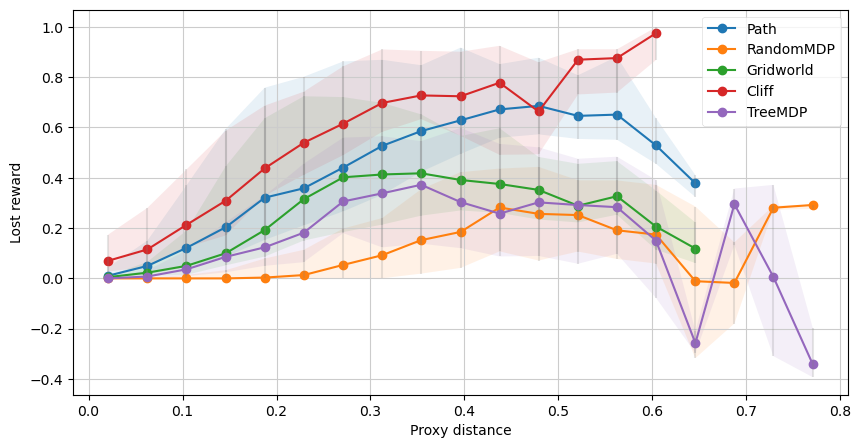
\includegraphics[width=1\linewidth]{lost_reward_plots/another_presentation_trend.png}
        \caption{}
        \label{fig:evaluation-theta}
    \end{subfigure}
    \caption{(a) Reward lost due to the early stopping ($\diamond$ show groups' medians). (b) The relationship between $\theta$ and the lost reward (shaded area between 25th-75th quantiles), aggregated into 25 buckets.}
\end{figure}
